\section{Iteración 5}


Para ampliar el conocimiento y dar un mayor abanico de opciones
a tener en cuenta en nuestro sistema de apoyo a la toma de decisión
se intenta pronosticar quien será el ganador de un asalto, de esa forma
el sistema podrá tenerlo en cuenta para dar una recomendación u otra.


Para el pronóstico se usarán técnicas de aprendizaje automático que se
verán mas adelante. Para poder aplicarlas hace falta una BBDD. Después de
una larga búsqueda fallida se decide crear nuestra propia BBDD sacando
la información de la página de la federación internacional de esgrima (FIE).

Todo lo ejecutado en esta iteración ha sido desarrollado con control de versiones
y se podrá consultar en el siguiente repositorio. Este sufrió modificaciones durante
el desarrollo y es por eso que el historico puede ser confuso. El repositorio se puede
consultar en el siguiente enlace \url{https://github.com/grego1201/MFT-API} o en la \hyperref[fig:Código QR repositorio api]{figura 5.12}.

\begin{figure}[htb]
  \centering
  \scalebox{.3}{
\includegraphics[width=0.8\linewidth]{QRApi}}
  \caption[Código QR repositorio api]{Código QR repositorio api}
  \label{fig:Código QR repositorio api}
\end{figure}

\subsection{Obtención BBDD}

En dicha página disponemos de toda la información de cada torneo acontecido
desde hace varios años con los resultados obtenidos en cada encuentro. Gracias
a esto podemos recopilar toda la información necesaria para poder obtener conocimiento
y transmitirlo a nuestro sistema para que este pueda nutrirse de él y que de este
modo sea mas amplio y fiable.

Para la obtención de datos se han realizado diferentes scripts desarrollados en
python mediante la técnica de scrapping, por lo que es posible que no sean funcionales
cuando esté leyendo esto dado que la página podría haber cambiado el diseño y/o
estructura, pero tan solo habría que adaptar parte de ellos para que vuelvan a
ser funcionales. La técnica de scrapping se basa en visitar la página web y
explorar su código para obtener la información de la misma.

Primero observamos la página y vimos como estaba estructurada. En este caso listaban
los torneos dando información sobre ellos como el tipo de torneo, género, arma, categoría,
etc. También usaban una paginación por lo que esto nos hacía pensar que había muchos tipos
de torneos y desde hace bastantes años. Cuando nos metimos a ver la estructura de dichos torneos
vimos como los registros eran diferentes, indicando solo la clasificación general algunos de ellos.
Esto sucedía sobre todo cuanto mas tiempo tuvieran, por lo que se decidió hacer una primera
criba y obtener aquellos a partir del 2015, que son aquellos en los que se empezaron a registrar
los resultados de las eliminatorias además de la clasificación general del torneo. Esta es la
información que nos interesa sacar, dado que con la clasificación general será algo más
complicado sacar conocimiento de esta para nuestro objetivo final. Mientras que con los
resultados obtenidos de cada enfrentamiento, junto a las características de cada tirador
como pueden ser ranking FIE, mano usada, edad y nacionalidad podremos sacar algo de
conocimiento con todo ello.

Con la primera criba hecha pasamos a sacar la información de cada torneo. Para ello exploraremos
la página con la información de cada competencia la cual contiene la clasificación general,
la cual no nos interesa almacenar. Por otro lado tenemos la fase de grupos o también
conocida como poules. Esta fase también la ignoraremos de momento pudiendo ser esta
información a analizar en un futuro. Ya sólo nos quedarían las fases eliminatorias o
cuadros de directas. Estos contienen el resultado del enfrentamiento: tocados dados por cada tirador,
quien ganó, el identificador de cada tirador y el tablón que se disputaba. Con esto la estructura de la BBDD
se queda de la siguiente forma (ver \hyperref[tab:Estructura BBDD Inicial iteracion5]{tabla 5.8}):

\begin{table}[]
  \centering
  \caption{Estructura BBDD Inicial}
  \label{tab:Estructura BBDD Inicial iteracion5}
  \begin{tabular}{|llll|}
    \hline \rowcolor[HTML]{C0C0C0}
    Campo & Tipo & Descripción & Ejemplo \\ \hline
    CompetitionID & String & Identificador de la competición & 2019-64 \\ \hline
    Tableu & Integer & 32 & 32 \\ \hline
    Competitor1 & String & Identificador del competidor 1 & /fencers/Anna-KOROLEVA-40351/ \\ \hline
    Competitor2 & String & Identificador del competidor 2 & /fencers/Kira-KESZEI-49034/ \\ \hline
    ResultCompetitor1 & String & Resultado del competidor 1 & V/15 \\ \hline
    ResultCompetitor2 & String & Resultado del competidor 2 & D/13 \\ \hline
  \end{tabular}
\end{table}

A continuación en la \hyperref[tab:Ejemplo BBDD inicial iteracion5]{tabla 5.9} se puede ver un ejemplo del estado inicial de la BBDD.

\begin{table}[]
  \centering
  \caption{Ejemplo BBDD inicial}
  \label{tab:Ejemplo BBDD inicial iteracion5}
  \begin{tabular}{|llllll|}
    \hline \rowcolor[HTML]{C0C0C0}
    CompetitionID & Tableu & Competitor1 & Competitor2 & ResultCompetitor1 & ResultCompetitor2 \\ \hline
    2019-64 & 32 & /fencers/Anna-KOROLEVA-40351/ & /fencers/Kira-KESZEI-49034/ & V/15 & D/13 \\ \hline
    2019-64 & 32 & /fencers/Greta-CECERE-45345/ & /fencers/Andreea-LUPU-37410/ & V/15 & D/12 \\ \hline
  \end{tabular}
\end{table}

Con esta información recopilada nos faltaría completarla. Para ello extrajimos en una BBDD
aparte todos los identificadores de los competidores, de esa forma podríamos extraer
sus características en una tabla aparte la cual recopile la información de todos
los competidores. Esta tabla contendrá la siguiente información de cada tirador:
identificador, edad, ranking, nacionalidad, mano dominante y arma. De tal forma
que la estructura se puede ver \hyperref[tab:Estructura BBDD tiradores]{tabla 5.10} y un ejemplo en la \hyperref[tab:Ejemplo BBDD tiradores]{tabla 5.11}.

\begin{table}[]
  \centering
  \caption{Estructura BBDD tiradores}
  \label{tab:Estructura BBDD tiradores}
  \begin{tabular}{|llll|}
    \hline \rowcolor[HTML]{C0C0C0}
    Campo & Tipo & Descripción & Ejemplo \\ \hline
    ID & String & Identificador del tirador & ADRIANA-MILANO-36467 \\ \hline
    Edad & Integer & Edad del tirador & 32 \\ \hline
    FieRanking & String & Ranking de campeonatos FIE del tirador & 1234 \\ \hline
    Nacionalidad & String & Nacionalidad del tirador & VENEZUELA \\ \hline
    Mano & String & Mano dominante del tirador & Right \\ \hline
    Arma & String & Arma principal del tirador & Sabre \\ \hline
  \end{tabular}
\end{table}

\begin{table}[]
  \centering
  \caption{Ejemplo BBDD tiradores}
  \label{tab:Ejemplo BBDD tiradores}
  \begin{tabular}{|llllll|}
    \hline
    \rowcolor[HTML]{C0C0C0}
    ID & Edad & FieRanking & Nacionalidad & Mano & Arma \\ \hline
    ADRIANA-MILANO-36467 & 21 & None & VENEZUELA & Right & Sabre \\ \hline
    AKHMETOV-Iskander-35108 & 22 & 82 & RUSSIA & Right & Foil \\ \hline
  \end{tabular}
\end{table}

Con toda la información recopilada juntaremos ambas BBDD de forma que
cruzando los datos de ambas podremos sustituir los identificadores del
de los tiradores de la primera BBDD con los datos recopilados de cada tirador.

De esta forma conseguiremos tener toda la información en una sola BBDD para
que los datos puedan ser comparados con mayor facilidad. La estructura final
de la BBDD se puede ver en la \hyperref[tab:estructura BBDD final]{tabla 5.12}.



\begin{longtable}{|p{3cm}p{2cm}p{6cm}p{3cm}|}
  \caption{Estructura BBDD final}
  \label{tab:estructura BBDD final}
  \endfirsthead
  \endhead

  \hline
  \rowcolor[HTML]{C0C0C0}
  Campo & Tipo & Descripción & Ejemplo \\ \hline
  ID & String & Identificador de la competición & ADRIANA-MILANO-36467 \\ \hline
  TABLEU & Integer & Tablón en el que se juega el asalto & 32 \\ \hline

  \rowcolor[HTML]{969696}
  C1\_ID & String & Identificador del primer tirador & Alexander-CHOUPENITCH-21765 \\ \hline
  \rowcolor[HTML]{969696}
  C1\_AGE & Integer & Edad del primer tirador & 32 \\ \hline
  \rowcolor[HTML]{969696}
  C1\_RANKING & Integer & Ranking del primer tirador & 10 \\ \hline
  \rowcolor[HTML]{969696}
  C1\_NATIONALITY & String & Nacionalidad del primer tirador & CZECH REPUBLIC \\ \hline
  \rowcolor[HTML]{969696}
  C1\_HANDNESS & String & Mano dominante del primer tirador & Right \\ \hline
  \rowcolor[HTML]{969696}
  C1\_WEAPON & String & Arma principal del primer tirador & Epee \\ \hline

  \rowcolor[HTML]{636363}
  C2\_ID & String & Identificador del segundo tirador & Alexander-CHOUPENITCH-21765 \\ \hline
  \rowcolor[HTML]{636363}
  C2\_AGE & Integer & Edad del segundo tirador & 32 \\ \hline
  \rowcolor[HTML]{636363}
  C2\_RANKING & Integer & Ranking del segundo tirador & 10 \\ \hline
  \rowcolor[HTML]{636363}
  C2\_NATIONALITY & String & Nacionalidad del segundo tirador & CZECH REPUBLIC \\ \hline
  \rowcolor[HTML]{636363}
  C2\_HANDNESS & String & Mano dominante del segundo tirador & Right \\ \hline
  \rowcolor[HTML]{636363}
  C2\_WEAPON & String & Arma principal del segundo tirador & Epee \\ \hline

  \rowcolor[HTML]{969696}
  RESULT\_C1 & String & Resultado del primer tirador & V/15 \\ \hline
  \rowcolor[HTML]{636363}
  RESULT\_C2 & String & Resultado del segundo tirador & D/7 \\ \hline
\end{longtable}

\subsection{Tratamiento BBDD}

El primer paso que daremos será añadir una columna numérica indicando quien
fue el ganador del encuentro. Esta contendrá 0 o 1 dependiendo de si ganó
el primer tirador o el segundo respectivamente. De esta forma será mas fácil
identificar quien de los dos tiradores ganó. La estructura del nuevo campo
se podrá ver en la \hyperref[tab:Estructura campo ganador]{tabla 5.13}. Para la obtención de este campo se exploró
el asalto correspondiente y se comprobó quien tenía dentro de su resultado
la letra \enquote{V} dado que esta es la que indicaba la victoria.

\begin{longtable}{|p{3cm}p{2cm}p{6cm}p{3cm}|}
  \caption{Estructura campo ganador}
  \label{tab:Estructura campo ganador}
  \endfirsthead
  \endhead

  \hline
  \rowcolor[HTML]{C0C0C0}
  Campo & Tipo & Descripción & Ejemplo \\ \hline
  WINNER & Integer & Este campo nos indicará quien ganó. Siendo 0 el primer tirador y 1 el segundo & 1 \\ \hline
\end{longtable}

Una vez calculado este campo ya no nos harían falta los campos de resultados
por lo que se procedió al borrado de los mismos.

El siguiente cambio que haremos será normalizar la BBDD. Esto se hace para
que los datos puedan ser comparados de una forma mas eficiente. Para ello
transformamos aquellas variables de texto a numéricas, de este modo serán
mas sencillos los cálculos estadísticos.

En nuestro caso tenemos la mano usada por el tirador y el arma usada por este.
Para ello seguiremos la transformación mostrada en la tabla \hyperref[tab:Tabla equivalencias mano]{5.14} y \hyperref[tab:Tabla equivalencias arma]{5.15} para
las equivalencias de mano y arma respectivamente. Esto se resume en
cambiar la mano dominante diestra por un valor de 0 mientras que la zurda será
sustituida por el valor 1. También cambiaremos las armas siendo el equivalente
de espada el 2, 1 para florete y restando el 0 para sable.

\begin{table}[]
  \centering
  \caption{Tabla equivalencias mano}
  \label{tab:Tabla equivalencias mano}
  \begin{tabular}{|ll|}
    \hline
    \rowcolor[HTML]{C0C0C0}
    Valor antiguo & Valor nuevo \\ \hline
    Right & 0 \\ \hline
    Left & 1 \\ \hline
  \end{tabular}
\end{table}

\begin{table}[]
  \centering
  \caption{Tabla equivalencias arma}
  \label{tab:Tabla equivalencias arma}
  \begin{tabular}{|ll|}
    \hline
    \rowcolor[HTML]{C0C0C0}
    Valor antiguo & Valor nuevo \\ \hline
    Sabre & 0 \\ \hline
    Foil & 1 \\ \hline
    Epee & 2 \\ \hline
  \end{tabular}
\end{table}

El siguiente paso era eliminar aquellas columnas que no nos sirvan. Para ello
primero quitaremos aquellas que puedan introducir mucho ruido y que son fáciles
de detectar como por ejemplo el identificador del tirador, puesto que es su nombre.
Este no tendrá ninguna relación con el resultado. Del mismo modo quitaremos las columnas
de resultados de resultados de ambos tiradores puesto que ya tenemos la de victoria.
Otro campo que está en la misma situación será el identificador de la competición.

Después de esto la estructura de la BBDD se puede ver en la \hyperref[tab:Estructura BBDD final postproceso]{tabla 5.16}.


\begin{longtable}{|p{3cm}p{2cm}p{6cm}p{3cm}|}
  \caption{Estructura BBDD final}
  \label{tab:Estructura BBDD final postproceso}
  \endfirsthead
  \endhead
  \hline \rowcolor[HTML]{C0C0C0}
  Campo & Tipo & Descripción & Ejemplo \\ \hline
  TABLEU & Integer & Tablón en el que se juega el asalto & 32 \\ \hline

  \rowcolor[HTML]{969696}
  C1\_AGE & Integer & Edad del primer tirador & 32 \\ \hline
  \rowcolor[HTML]{969696}
  C1\_RANKING & Integer & Ranking del primer tirador & 10 \\ \hline
  \rowcolor[HTML]{969696}
  C1\_NATIONALITY & String & Nacionalidad del primer tirador & CZECH REPUBLIC \\ \hline
  \rowcolor[HTML]{969696}
  C1\_HANDNESS & String & Mano dominante del primer tirador & Right \\ \hline
  \rowcolor[HTML]{969696}
  C1\_WEAPON & String & Arma principal del primer tirador & Epee \\ \hline

  \rowcolor[HTML]{636363}
  C2\_AGE & Integer & Edad del segundo tirador & 32 \\ \hline
  \rowcolor[HTML]{636363}
  C2\_RANKING & Integer & Ranking del segundo tirador & 10 \\ \hline
  \rowcolor[HTML]{636363}
  C2\_NATIONALITY & String & Nacionalidad del segundo tirador & CZECH REPUBLIC \\ \hline
  \rowcolor[HTML]{636363}
  C2\_HANDNESS & String & Mano dominante del segundo tirador & Right \\ \hline
  \rowcolor[HTML]{636363}
  C2\_WEAPON & String & Arma principal del segundo tirador & Epee \\ \hline

  \rowcolor[HTML]{969696}
  WINNER & Integer & Este campo nos indicará quien ganó. Siendo 0 el primer tirador y 1 el segundo & 1 \\ \hline
\end{longtable}

\newpage

\subsection{Extraer conocimiento de los datos}

Una vez que tenemos la BBDD normalizada el siguiente paso será buscar relaciones
entre los datos de modo que se pueda extraer conocimiento de estos mismos y de
esa forma poder mejorar nuestro sistema. El objetivo inicial es el de obtener
un pronóstico de quien ganará en un enfrentamiento directo. De este modo podremos
completar nuestro sistema adaptando una táctica mas defensiva en función
del resultado. No podremos ser agresivos o intentar movimientos que no tengamos afianzados
ante un rival que es muy probable que nos gane. En este caso mencionado antes lo mejor
será asegurar y llevarnos el asalto a nuestro terreno.

Como hemos mencionado antes el problema que tenemos antes es el de intentar pronosticar
el vencedor ante un enfrentamiento entre dos tiradores. Eso denota a que los resultados
serán ganador uno o ganador otro. Por ende nos enfrentamos ante un problema de clasificación
binaria. Clasificación puesto que los resultados estarán en grupos y binario porque el número
de posibles opciones son dos en este caso en concreto denotado por el objetivo final.

Además podremos aplicar técnicas de aprendizaje supervisado, dado que tenemos un conjunto de datos
previamente etiquetados gracias a todo el trabajo realizado anteriormente. Además podemos
estar seguros de que el etiquetado es el correcto, puesto que la veracidad de estos datos
es completa. Ante un problema de tales características los algoritmos más utilizados suelen ser
arboles de decisión, clasificación de Naïve Bayes, regresión por mínimos cuadrados, regresión
logística, Support Vector Machines (SVM) y métodos ensemble (conjuntos de clasificadores).

Para elegir alguno de estos podemos seguir la chuleta que nos proporciona scikit-learn la cuál se
puede encontrar en la \hyperref[fig:Chuleta decisión algoritmo ML]{figura 5.13}.

\begin{figure}[htb]
  \centering
    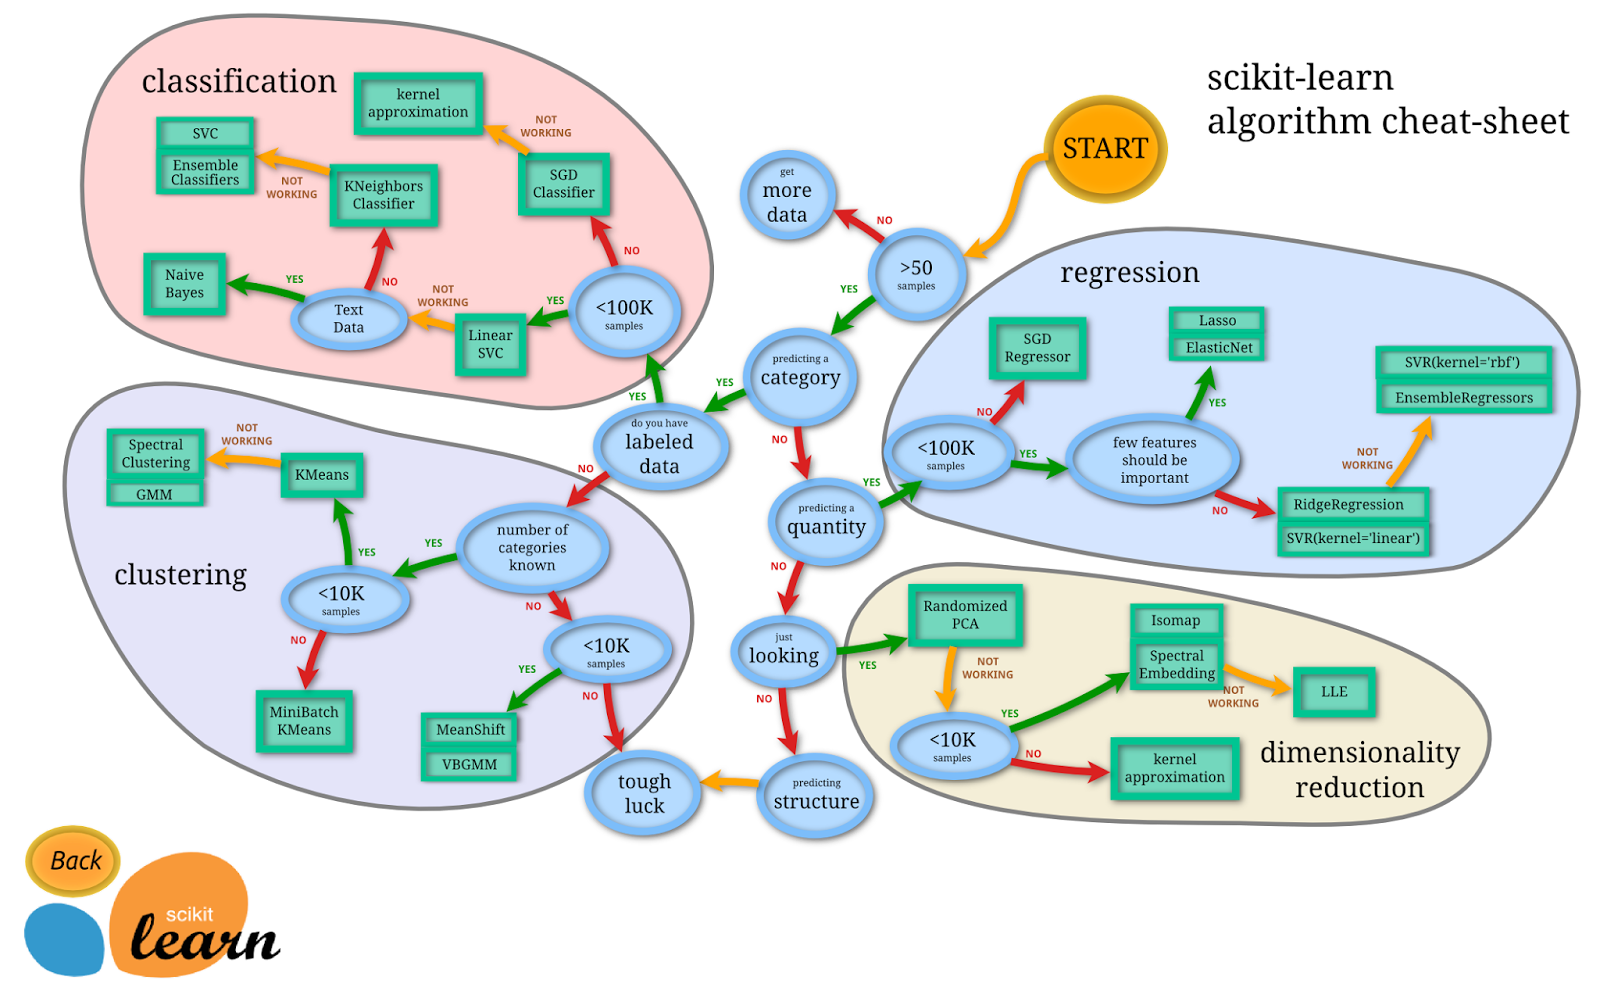
\includegraphics[width=0.8\linewidth]{ml_map}
  \caption[Chuleta decisión algoritmo ML]{Chuleta decisión algoritmo ML}
  \label{fig:Chuleta decisión algoritmo ML}
\end{figure}

Siguiendo esta chuleta y siguiendo el flujo veremos que algoritmo nos recomienda.
Para la primera pregunta la respuesta sería sí, dado que tenemos mas de 50 ejemplos.
Como hemos visto antes intentamos predecir una categoría y además tenemos los datos
etiquetados, las dos siguientes respuestas serán afirmativas. La siguiente pregunta
es que si tenemos menos de 100.000 ejemplos y en este caso también será afirmativa.
Nuestra BBDD se compone de 25.045 registros.

Para aplicar los algoritmos usaremos la librería scikit-learn dado que nos proporciona
todas las herramientas que necesitaremos para aplicarlos.

El primer algoritmo que deberemos aplicar según la chuleta será linear SVC. En caso
de que no funcione seguiremos con la chuleta.

Después de varias pruebas el mejor resultado obtenido fue de un 63.78 \% de acierto. Es
algo bajo por lo que nos disponemos a buscar alternativas. El código utilizado fue el siguiente:

\begin{lstlisting}[language=python]
LSVC = LinearSVC(dual=False, fit_intercept=False)

LSVC.fit(x1,y1)
y2_LR_model = LSVC.predict(x2)
print("LR Accuracy :", accuracy_score(y2, y2_LR_model))
\end{lstlisting}

El siguiente a probar será un clasificador por cercanía de vecinos o mas conocido como KNN.

Para ello lo primero será averiguar el número de vecinos óptimo. El plan que seguimos
fue probar diferentes opciones y ver cual era la que nos daba una mayor precisión. El resultado
que obtuvimos fue que el mejor valor era de 53 con una precisión del 0.6460194963444355\%.
En la \hyperref[fig:Gráfica obtención K]{figura 5.14} se puede ver la gráfica comparativa.

\begin{figure}[htb]
  \centering
    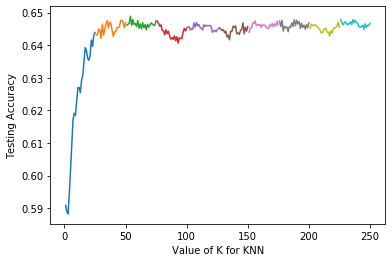
\includegraphics[width=0.65\linewidth]{best_k}
  \caption[Gráfica obtención K]{Gráfica obtención K}
  \label{fig:Gráfica obtención K}
\end{figure}

Este fue el código utilizado:

\begin{lstlisting}
iterations = range(0, 10)
for i in iterations:
    k_range = range((i * 25) + 1, (i * 25) + 26)
    scores = []
    for k in k_range:
        knn = KNeighborsClassifier(n_neighbors=k, n_jobs=5)
        knn.fit(X_train, y_train)
        y_pred = knn.predict(X_test)
        scores.append(metrics.accuracy_score(y_test, y_pred))

    if max_score < max(scores):
        max_score = max(scores)
        max_k = scores.index(max(scores)) + (i * 25)

    plt.plot(k_range, scores)

plt.xlabel('Value of K for KNN')
plt.ylabel('Testing Accuracy')
plt.show()
plt.close()
print ("max_score:")
print (max_score)
print ("max_k:")
print (max_k)
\end{lstlisting}

El siguiente parámetro a probar será el número de hijos que deberá tener
cada hoja en la exploración. Para ello lanzaremos el siguiente código cuyo
resultado se puede puede observar en la \hyperref[fig:Gráfica obtención leaf size]{figura 5.15}. El resultado que obtuvimos
fue que le mejor valor estaba en 8. Este valor nos proporcionaba una precisión
de 0.6436839967506093\%. 

\begin{figure}[htb]
	\centering
	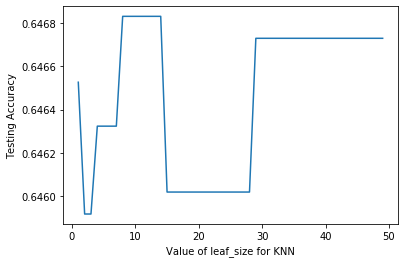
\includegraphics[width=0.65\linewidth]{best_leaf_size}
	\caption[Gráfica obtención leaf size]{Gráfica obtención leaf size}
	\label{fig:Gráfica obtención leaf size}
\end{figure}

El código utilizado fue el siguiente:

\begin{lstlisting}
k_range = range(1, 60)
scores = []

max_score = 0
max_k = 0

for i in k_range:
    knn = KNeighborsClassifier(n_neighbors=53, n_jobs=5, leaf_size=i)
    knn.fit(X_train, y_train)
    y_pred = knn.predict(X_test)
    score = metrics.accuracy_score(y_test, y_pred)
    scores.append(score)
    if max_score < score:
        max_score = score
        max_k = i

plt.plot(k_range, scores)
plt.xlabel('Value of leaf_size for KNN')
plt.ylabel('Testing Accuracy')
plt.show()
plt.close()

print ("max leaf size")
print ("max_score:")
print (max_score)
print ("max_k:")
print (max_k)
\end{lstlisting}



La siguiente variable a probar sería el valor de P, el cuál representará el power.
Repetiremos el mismo proceso para esta variable. El mejor resultado lo obtuvimos con
el valor de 1 con un porcentaje de 0.6487611697806661\%. La gráfica se puede observar
en la \hyperref[fig:Gráfica obtención p]{figura 5.16}.

\begin{figure}[htb]
	\centering
	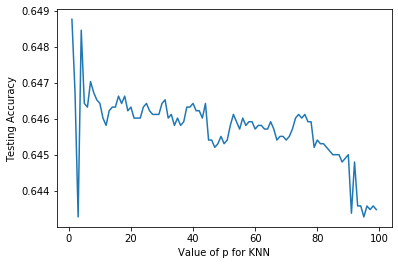
\includegraphics[width=0.65\linewidth]{best_p}
	\caption[Gráfica obtención p]{Gráfica obtención p}
	\label{fig:Gráfica obtención p}
\end{figure}


El código utilizado es el siguiente:
\begin{lstlisting}
k_range = range(1, 100)
scores = []

max_score = 0
max_k = 0

for i in k_range:
    knn = KNeighborsClassifier(n_neighbors=53, n_jobs=5, leaf_size=30, p=i)
    knn.fit(X_train, y_train)
    y_pred = knn.predict(X_test)
    score = metrics.accuracy_score(y_test, y_pred)
    scores.append(score)
    if max_score < score:
        max_score = score
        max_k = i

plt.plot(k_range, scores)
plt.xlabel('Value of p for KNN')
plt.ylabel('Testing Accuracy')
plt.show()
plt.close()

print ("max p value")
print ("max_score:")
print (max_score)
print ("max_k:")
print (max_k)
\end{lstlisting}


Finalmente el modelo tendrá una precisión de 0.6487611697806661\% el cuál es algo
aceptable para los datos que tenemos. El modelo es el siguiente:

\begin{lstlisting}
knn = KNeighborsClassifier(n_neighbors=53, n_jobs=5, leaf_size=29, p=1)

knn.fit(X_train, y_train)
y_pred = knn.predict(X_test)
print (metrics.accuracy_score(y_test, y_pred))
\end{lstlisting}

Puesto que se podría llegar a encontrar una solución mas óptima pero habría que probar
por fuerza bruta preparamos un algoritmo que pruebe estas tres variables entre los rangos
que vimos que podrían ser válidos. Estos rangos son de 1 a 2500 para número de vecinos,
de 1 a 60 para el tamaño de hoja y de 1 a 20 para el valor de p.

Dicho algoritmo lo podemos encontrar en el \hyperref[cap:Algoritmo valores KNN]{anexo G}.

Los resultados obtenidos se consiguieron después de mas de dos días de procesamiento.
Para el valor de K se obtuvo que el valor de 56, siendo este el número de grupos. Por otro lado
el tamaño máximo de hoja será de 29. Por último el valor de p será de 5. Con esto se consiguió
una precisión de 0.652315190901706\%, consiguiendo una mejora de 0.05 puntos de precisión.

Esto mereció la pena debido a que teníamos bastante tiempo para lanzar el algoritmo. Puesto que
los resultados ya se han obtenido y son mejores que los obtenidos con anterioridad nos
quedaremos con ellos.

\subsection{Usar conocimiento en aplicación}

Con el modelo optimizado lo máximo posible y obtenido un resultado mas que aceptable
para los datos que manejamos podremos incluirlo en nuestro sistema. Para ello aprovecharemos
que el modelo nos proporciona el porcentaje de probabilidad de que gane cada uno, lo cual nos
dará la oportunidad de poder crear reglas en función de las probabilidades. Para poder acceder
a ello crearemos una API a la cual llamaremos cada vez que queramos realizar la consulta.

Esta API estará realizada en python con flask la cual solo tendrá una llamada que devolverá
la probabilidad de que gane cada uno de los tiradores. En los parámetros de esta API estarán
incluidas las características del asalto, es decir, características de cada tirador y tablón.
De esta forma podremos llamar al modelo, que este haga la predicción y que nos
devuelva el resultado.

El endpoint llamado con curl será de la siguiente manera:

\begin{lstlisting}
curl -X GET https://mftapi.herokuapp.com/predict/ -d "tableu=16&fencer1_age=26&fencer1_ranking=33& fencer1_handness=0&fencer1_weapon=1.0&fencer2_age=44& fencer2_ranking=99999999&fencer2_handness=0& fencer2_weapon=1.0"
\end{lstlisting}

Los parámetros con sus características se podrán consultar en la \hyperref[tab:Parmetros peticion prediccion]{tabla 5.17}.


\begin{longtable}{llllll}
	\caption{Parámetros petición predicción}
	\label{tab:Parmetros peticion prediccion}

  \endfirsthead
  \endhead
  Parámetro & Descripción & Tipo & Requerido & Valores admitidos & Ejemplo \\ \hline
  \multicolumn{1}{l|}{tableu} & \multicolumn{1}{l|}{Tablón encuentro} & Integer & Si & \{2, 4, 8, 16, 32, 64, ...\} & 2 \\ \hline
  \multicolumn{1}{l|}{fencer1\_age} & \multicolumn{1}{l|}{Edad tirador 1} & Integer & Si & \{1, inf\} & 26 \\
  \multicolumn{1}{l|}{fencer1\_ranking} & \multicolumn{1}{l|}{Ranking tirador 1} & Integer & Si & \{1, inf\} & 33 \\
  \multicolumn{1}{l|}{fencer1\_handness} & \multicolumn{1}{l|}{Mano tirador 1 (0 derecha, 1 izquierda)} & Integer & Si & \{{[}\}0, 1\{{]}\} & 0 \\
  \multicolumn{1}{l|}{fencer1\_weapon} & \multicolumn{1}{l|}{Arma tirador 1 (0 florete, 1 sable, 2 espada)} & Integer & Si & \{{[}\}0, 1, 2\{{]}\} & 1 \\ \hline
  \multicolumn{1}{l|}{fencer2\_age} & \multicolumn{1}{l|}{Edad tirador 2} & Integer & Si & \{1, inf\} & 44 \\
  \multicolumn{1}{l|}{fencer2\_ranking} & \multicolumn{1}{l|}{Ranking tirador 2} & Integer & Si & \{1, inf\} & 9999999999 \\
  \multicolumn{1}{l|}{fencer2\_handness} & \multicolumn{1}{l|}{Mano tirador 2 (0 derecha, 1 izquierda)} & Integer & Si & \{{[}\}0, 1\{{]}\} & 0 \\
  \multicolumn{1}{l|}{fencer2\_weapon} & \multicolumn{1}{l|}{Arma tirador 2 (0 florete, 1 sable, 2 espada)} & Integer & Si & \{{[}\}0, 1, 2\{{]}\} & 1
\end{longtable}

Para la implementación de dicha API se utilizó el lenguaje de programación Python 3.6.9 para
aprovechar el código utilizado a la hora de entrenar el modelo anterior. Las librerías
utilizadas para las peticiones fueron Flask junto a GUnicorn para darle una interfaz web.


Por otro lado el hosting utilizado volvió a ser Heroku dado que tiene un límite de cinco
proyectos por cuenta de forma gratuita. Esto nos permite ahorrar costes en el proyecto
Además del endpoint mencionado anteriormente tendremos otro para que haga una llamada vacía
la cual será la encargada de levantar el servidor, puesto que el programa gratuito apaga
las máquinas a los treinta minutos de no recibir peticiones. Cuando accedan a la página, una
vez por sesión hará la llamada asíncrona a dicho endpoint, de este modo la máquina de la API
se irá levantando mientras el usuario navega por la web o rellena el formulario. De este modo
bajaremos el tiempo de espera del usuario de treinta segundos aproximados que tarda la máquina en
estar lista a esos treinta segundos menos el tiempo que tarde en rellenar el formulario, siendo
este una media de 20 segundos. El mínimo de tiempo que estará el usuario esperando será de tres
segundos puesto que es lo que tarda el endpoint de predicción en llevar a cabo la petición.

Para adaptar el proyecto a los requirimientos que tiene heroku fue necesario crear un fichero
\textit{requirements.txt} con las dependencias de librerías. El contenido de dicho documento
se puede ver a continuación:

\lstinputlisting[]{code/requirements.txt}

Así mismo Heroku también necesita un fichero con el que indicar al servidor que comando
utilizar para arrancar. Este comando se tiene que guardar en un fichero llamado
\textit{Procfile} cuyo contenido se puede ver a continuación:

\lstinputlisting[]{code/Procfile}

% El código utilizado por el servidor se puede ver en el anexo G.

Una vez con todo este proceso hecho, se mantuvo una conversación con el experto mediante mensajería
instantánea. En dicha conversación se volvieron a destacar conceptos ya mencionados anteriormente
como la confianza del tirador, tanto la de uno mismo como la del rival. También menciono cuanto
había que arriesgar en función de la diferencia de nivel entre ambos tiradores. Pudiendo
arriesgar más cuanta mas haya, siempre que esté a tu favor. En caso contrario se procurará ser
lo mas conservador posible. Al ser conservadores el tirador irá cogiendo confianza con los
tocados que mejor le salen y de esta forma podrá llevar el asalto a su terreno.

Esto nos llevó a ampliar las variables del sistema experto añadiendo un parámetro más: diferencia
de nivel. Este parámetro será un número entre 0 y 100 representando porcentajes de probabilidad
de que gane el primer tirador. La tabla objeto atributo valor de los nuevos atributos se puede
ver en la \hyperref[tab:Tabla objeto atributo y valor victoria]{tabla 5.18}.

\begin{longtable}{lll}
  \caption{Tabla objeto atributo y valor victoria}
  \label{tab:Tabla objeto atributo y valor victoria}

  \endfirsthead
  \endhead

  Objeto & Atributo & Valor \\ \hline
  \multicolumn{1}{l|}{Tirador} & Probabilidad victoria tirador 1 & [0, 100]\%
\end{longtable}

Esta variable será tenida en cuenta para el siguiente árbol que representará
cuanto riesgo ha de tomar un esgrimista en la pista. Dicho árbol se puede
ver en la \hyperref[fig:Mapa conocimiento arriesgar]{figura 5.17}.

\begin{figure}[htb]
  \centering
    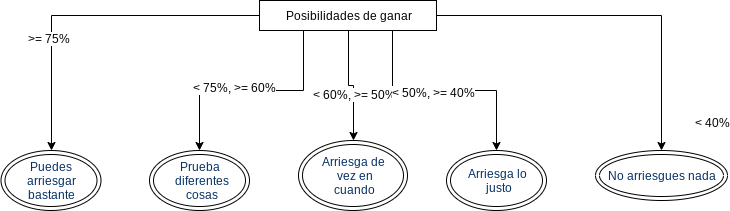
\includegraphics[width=0.8\linewidth]{mapaArriesgar}
  \caption[Mapa conocimiento arriesgar]{Mapa conocimiento arriesgar}
  \label{fig:Mapa conocimiento arriesgar}
\end{figure}

La representación del mapa es que si la estadística juega totalmente a nuestro favor
podremos arriesgar bastante, dado que en teoría podremos tomar las riendas del asalto
en cualquier momento. Si se decantan hacia nuestro lado, pero no del todo nos podremos
permitir arriesgar de vez en cuando, pero sin tomarnos demasiadas licencias, puesto que
nos costará mas remontar el asalto si se complica. En caso de que las cosas estén empatadas
podremos probar de vez en cuando, pero siendo la mayor parte del tiempo conservadores. En
caso de que se decanten un poco hacia su lado las cosas tendremos que arriesgar en las ocasiones
mas claras. Por último si se decantan hacia su lado no podremos arriesgar nada, puesto que lo normal
es que cualquier error sea pagado muy caro.
